\documentclass{report}
\usepackage{polyglossia}
\usepackage{fixlatvian}
\usepackage{graphicx}
\usepackage{circuitikz}
\usepackage{tabularx}
\usepackage{verbatim}
\usepackage{float}
\usepackage{pgfplots}
\graphicspath{{bildes/}}
\title{Laboratorijas darba atskaite}
\author{Rūdolfs Grīnbergs}

\begin{document}
\maketitle
%=============================
\chapter{Teorētiskā daļa}
\section{Ķēdes aprēķins}
Sprieguma avota V1 vērtība ir studenta apliecības pēdējie trīs cipari dalīti ar 10. R1 ir apliecības pēdējo 3 ciparu otrais numurs + 1, R2 ir apliecības numura pēdējais cipars + 1. Apliecības numurs: 171REB092. Sprieguma kritumu vērtības $U_{R1}$ un $U_{R2}$ tika aprēķinātas pēc formulas:\\ $$U_{R1}=\frac{R1}{R1+R2}\cdot V1$$\\
Rezultāti ir apskatāmi tabulā \ref{table:ta} un shēma ir aplūkojama attelos \ref{fig:sh} un \ref{fig:sh2} Atskaite tika sagatavota izmantojot sharelatex.com \cite{1} \cite{2} piedāvātos mācību palīglidzekļus, uz kuriem saites ir pieejamas bibliogrāfijas sarakstā, kā arī citus interneta resursus.


\begin{table}[h]
\centering
\begin{tabular}[h]{|c|c|}
\hline
$R1$ & 10 $\Omega$\\
\hline
$R2$ & 3 $\Omega$\\
\hline
$V1$ & 9.2 V\\
\hline
$U_{R_1}$ & 9.2 V\\
\hline
$U_{R_2}$ & 2.76 V\\
\hline
\end{tabular}
\caption{}
\label{table:ta}
\end{table}



\begin{figure}[t]
\centering
\begin{circuitikz}
\draw
(0,0) to[european voltage source, l_=$V_1$] (0,4)
to[european resistor, l_=$R_1$] (4,4)
to[european resistor, l_=$R_2$] (4,0) -- (0,0)
;
\end{circuitikz}
\caption{}
\label{fig:sh}
\end{figure}

\begin{figure}[!b]
\centering
\begin{tikzpicture}
\begin{axis}[
    title={$U_{R_{2}}=f(R_2)$},
    xlabel={$R_2$ [$\Omega$]},
    ylabel={$U_{R_{2}}$ [V]},
    xmin=5, xmax=50,
    ymin=0, ymax=15,
    xtick={0,10,20,30,40,50},
    ytick={0,5,10,15},
    ymajorgrids=true,
    xmajorgrids=true,
    grid style=dashed,
]
\addplot[color=blue,]
    coordinates {
    (5,3.07)(10,4.6)(15,5.52)(20,6.13)(25,6.57)(30,6.9)(35,7.16)(40,7.36)(45,7.53)(50,7.67)
    };
\end{axis}
\end{tikzpicture}
\caption{}
\label{fig:gr}
\end{figure}
%=============================
\chapter{Praktiskā daļa}
\section{Darbs ar GEDA programmām}
\subsection{Darbs ar gschem}
\begin{figure}[h]
    \centering
    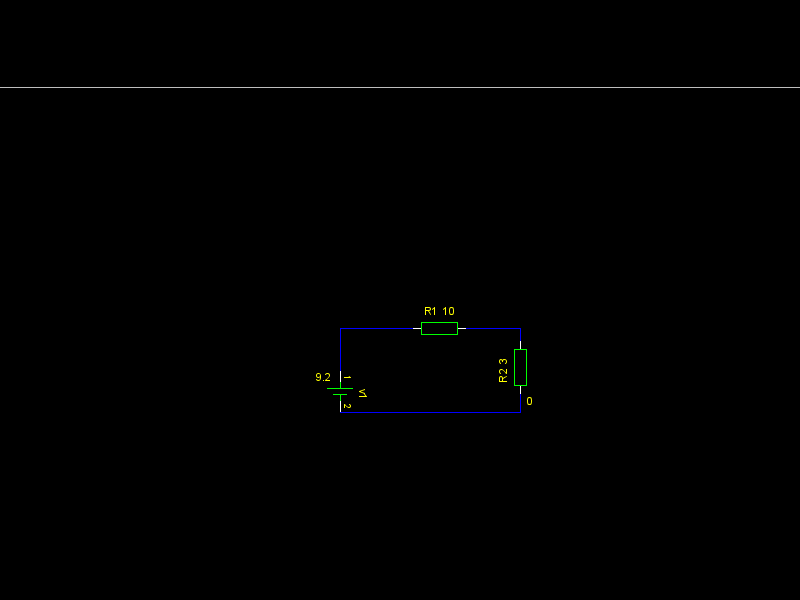
\includegraphics{01.png}
    \caption{}
    \label{fig:sh2}
\end{figure}

\newpage
\subsection{Darbs ar gnetlist}
\verbatiminput{bildes/01.net}

\subsection{Darbs ar ngspice}
Skatīt attēlus \ref{fig:2.1} un \ref{fig:2.2} 
\begin{figure}[!h]
    \centering
    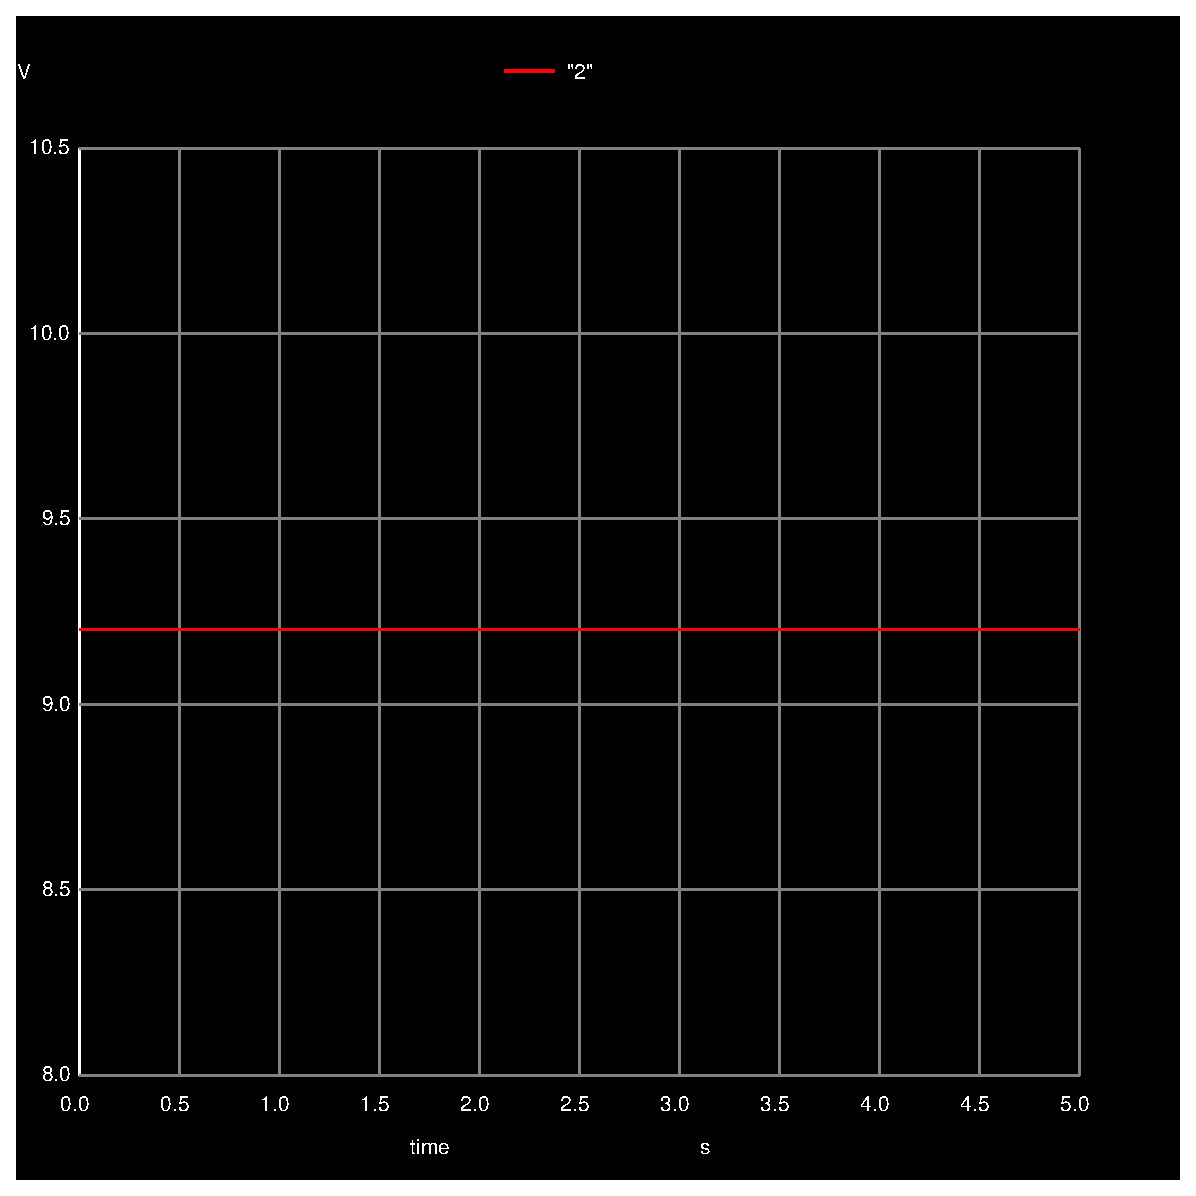
\includegraphics[width=10cm]{012.ps}
    \caption{Spriegums 1.vadā}
    \label{fig:2.1}
    \end{figure}
 \begin{figure}[t]
 \centering
    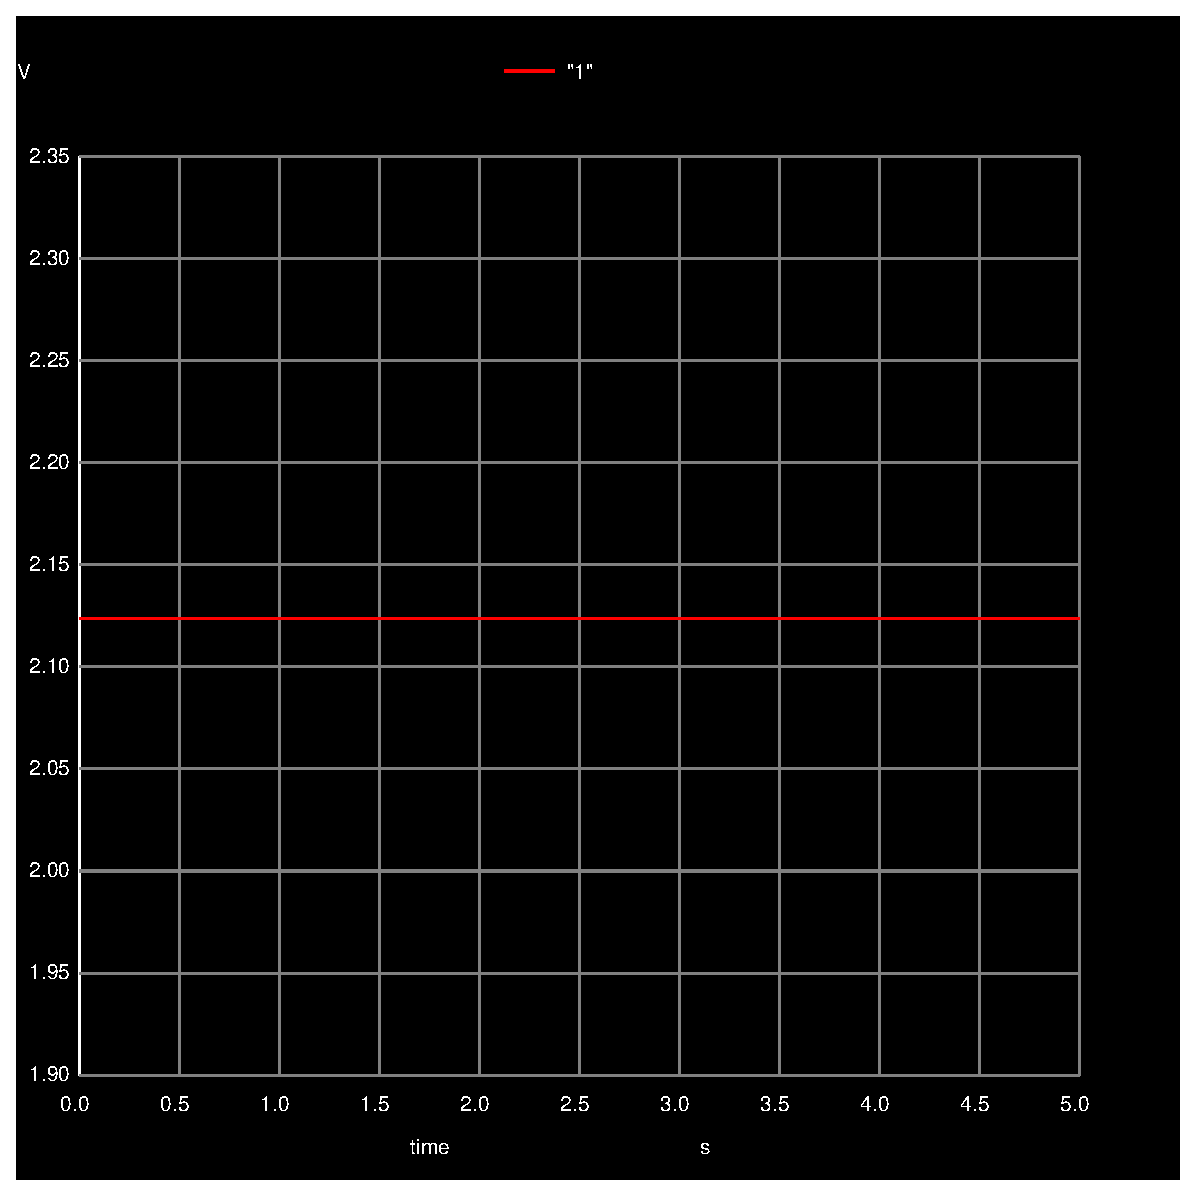
\includegraphics[width=10cm]{011.ps}
    \caption{Spriegums 2.vadā}
    \label{fig:2.2}
\end{figure}
\newpage

\section{Darbs ar QUCS programmām}
\begin{figure}[!h]
    \centering
    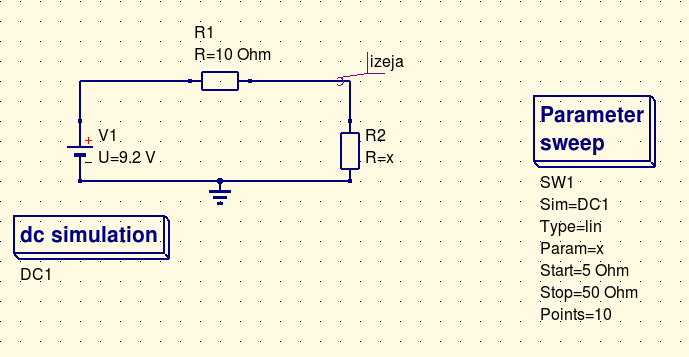
\includegraphics[width=\textwidth, height=\textheight, keepaspectratio]{QUCS.png}
    \caption{QUCS shēma}
    \label{fig:2.3}
    \end{figure}
 
\begin{figure}[t] 
\centering
    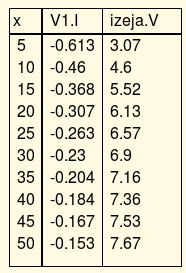
\includegraphics[width=\textwidth, height=220 pt, keepaspectratio]{sweep.png}
    \caption{Sweep simulācijas tabula}
    \label{fig:2.4}
\end{figure}

\newpage

\begin{figure}[h]
\centering
 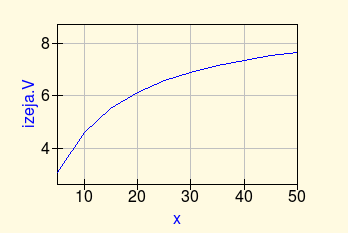
\includegraphics[width=\textwidth, height=\textheight, keepaspectratio]{Graf.png}
    \caption{Līdzstrāvas simulācijas grafiks}
    \label{fig:2.5}
\end{figure}
\label{s_nobeigums}

\begin{thebibliography}{9}
\bibitem{1} 
\textit{CircuiTikz package.} [Skatīts 2018. gada 27. martā].
Pieejams: http://www.sharelatex.com/learn/CircuiTikz\_{}package

\bibitem{2} 
\textit{Pgfplots package.} [Skatīts 2018. gada 27. martā].
Pieejams: http://www.sharelatex.com/learn/Pgfplots\_{}package
 
\end{thebibliography}

\end{document}
